\documentclass{article}

% formato
\usepackage[margin = 1.5cm, letterpaper]{geometry}
\usepackage[utf8]{inputenc}
\usepackage{graphicx}% http://ctan.org/pkg/graphicx
\usepackage{array}

% autómatas
\usepackage{tikz}
\usetikzlibrary{automata, positioning}

%formato ecuaciones
\usepackage{amsmath}

% símbolos
\usepackage{amssymb}

% manejo de tablas
\usepackage{float}

\begin{document}
    \title{
        Lenguajes de Programación \\
        Ejercicio Semanal 3
    }

    \author{
        Sandra del Mar Soto Corderi \\
        Edgar Quiroz Castañeda
    }

    \date{
        22 de agosto del 2019
    }
    
    \maketitle

    \begin{enumerate}
        \item {
            Responde cada inciso a partir de la siguiente expresión $e$
                            
            	$\texttt{let x = let y = 3 in 2 + y end in}$\\
            	$\textcolor{white}{eas}\texttt{let w = let y = 2 in y * 5 end in}$\\
            	$\textcolor{white}{easypie}\texttt{let y = w / x in y + x end + 2}$\\
            	$\textcolor{white}{easypie}\texttt{end}$\\
            	$\texttt{end}$\\
            
            
            \begin{enumerate}
            	\item { Llenar la siguiente tabla con base en $e$. El orden de las expresiones let es, por supuesto, el orden de lectura
            		como texto.
            		
            		\begin{table}[H]
            			\centering
            			\begin{tabular}{|l|l|l|l|}
            				\hline
            				let & variable ligada & expresión a ligar & alcance del let \\ \hline
            				1   & x               & 
            				\begin{minipage}{.3\textwidth}
            					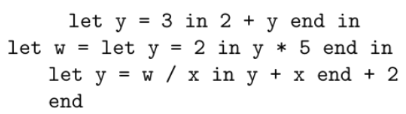
\includegraphics[width=\linewidth, height=.25\linewidth]{x1.png}
            				\end{minipage}
            			     & \begin{minipage}{.3\textwidth}
            			         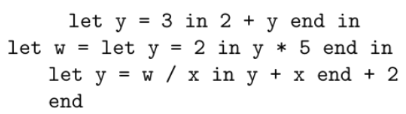
\includegraphics[width=\linewidth, 
            			        height=.25\linewidth]{x1.png}
            		       \end{minipage}                \\ \hline
            				2   & y               & \begin{minipage}{.3\textwidth}
            					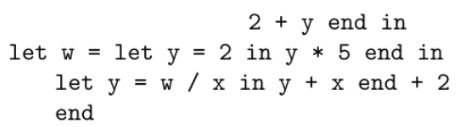
\includegraphics[width=\linewidth, height=.25\linewidth]{y1.png}
            				\end{minipage}                  &  \begin{minipage}{.3\textwidth}
            				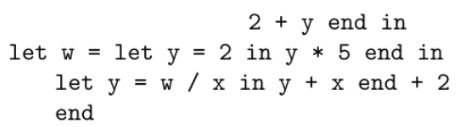
\includegraphics[width=\linewidth, height=.25\linewidth]{y1.png}
            			\end{minipage}               \\ \hline
            				3   & w               & \begin{minipage}{.3\textwidth}
            					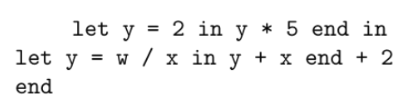
\includegraphics[width=\linewidth, height=.25\linewidth]{w1.png}
            				\end{minipage}                  &  \begin{minipage}{.3\textwidth}
            				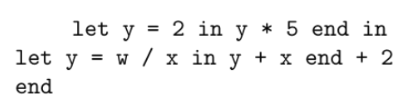
\includegraphics[width=\linewidth, height=.25\linewidth]{w1.png}
            			\end{minipage}               \\ \hline
            				4   & y               &  \begin{minipage}{.3\textwidth}
            					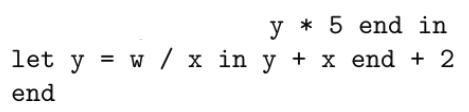
\includegraphics[width=\linewidth, height=.25\linewidth]{y2.png}
            				\end{minipage}                 & \begin{minipage}{.3\textwidth}
            				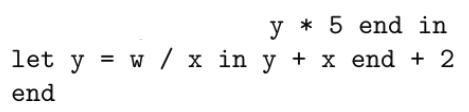
\includegraphics[width=\linewidth, height=.25\linewidth]{y2.png}
            			\end{minipage}                \\ \hline
            				5   & y               &  $x+y$                 &  $x+y$               \\ \hline
            			\end{tabular}
            		\end{table}
            	}
            \item {
            Encuentra la representación en la sintaxis abstracta de orden superior de $e$. Está permitido usar sintaxis concreta para operaciones y números.
            
        	$let \ (let\ num[3],\ y.suma(num[2], y)),\ x.let(let (num[2],\ y.prod(y, num[5]),\ w.suma(let(div(w,x),\ y.suma(y,x), num[2]))$\\
        	
        	
        	}
        	\item{
        	Encuentra una expresión $e'$ que sea $\alpha$-equivalente a $e$ y en donde todas las variables ligadas tengan distinto nombre.\\
        	
        	$e' = \texttt{let x = let y = 3 in 2 + y end in}$\\
        	$\textcolor{white}{eas}\texttt{let w = let z = 2 in z * 5 end in}$\\
        	$\textcolor{white}{easypie}\texttt{let a = w / x in a + x end + 2}$\\
        	$\textcolor{white}{easypie}\texttt{end}$\\
        	$\texttt{end}$\\
        	
        	}
        	\item {
        	¿Cuál es el valor de $e$? Explica como se llego al resultado.\\
        	
        	$e=9$
        	
        	Utilizando los juicios de transición que vienen en las notas, tenemos :\\
        	      	
        	\begin{align*}
        	&\texttt{let} \ x = \texttt{let} \ y = 3 \ \texttt{in} \ 2 + y \ \texttt{end} \  \ \texttt{in} \\\
        	&\texttt{let} \ w = \texttt{let} \ y = 2 \ \texttt{in} \ y * 5 \ \texttt{end} \  \ \texttt{in} \\\
        	&\texttt{let} \ y = w / x \ \texttt{in} \ y + x \ \texttt{end} \  + 2\\
        	&\ \texttt{end} \ \\
        	&\ \texttt{end} \ \\
        	&\rightarrow (eletf) \\
        	&\texttt{let} \ x = (2 + y)[y:=3] \ \ \texttt{in} \\
        	&\texttt{let} \ w =  (y * 5)[y:=2] \ \texttt{in} \\
        	&\texttt{let} \ y = w / x \ \texttt{in} \ y + x \ \texttt{end} \  + 2\\
        	&\ \texttt{end} \ \\
        	&\ \texttt{end} \ \\
        	&= \\
        	&\texttt{let} \ x = (2 + 3) \ \ \texttt{in} \\
        	&\texttt{let} \ w =  (2 * 5) \ \texttt{in} \\
        	&\texttt{let} \ y = w / x \ \texttt{in} \ y + x \ \texttt{end} \  + 2\\
        	&\ \texttt{end} \ \\
        	&\ \texttt{end} \ \\
        	&\rightarrow (esumf), (eprodf), (eleti) \\
        	&\texttt{let} \ x = 5 \ \ \texttt{in} \\
        	&\texttt{let} \ w =  10 \ \texttt{in} \\
        	&\texttt{let} \ y = w / x \ \texttt{in} \ y + x \ \texttt{end} \  + 2\\
        	&\ \texttt{end} \ \\
        	&\ \texttt{end} \ \\
        	&\rightarrow (eletf) \\
        	&(\texttt{let} \ y = w / x \ \texttt{in} \ y + x \ \texttt{end} \  + 2)
        	[x := 5, w := 10]\\
        	&= \\
        	&\texttt{let} \ y = (w / x)[x := 5, w := 10] \ \texttt{in} \ 
        	(y + x) [x := 5, w := 10] \ \texttt{end} \  + 2 \\
        	&\rightarrow (eleti) \\
        	&\texttt{let} \ y = 10 / 5 \ \texttt{in} \ y + 5\ \texttt{end} \  + 2 \\
        	&\rightarrow (eprodf), (eleti) \\
        	&\texttt{let} \ y = 2 \ \texttt{in} \ y + 5\ \texttt{end} \  + 2 \\
        	&\rightarrow (eletf) \\
        	&(y+5)[y:=2] + 2 \\
        	&= \\
        	& 2 + 5 + 2 \\
        	&\rightarrow (esumf) \\
        	& 9
        	\end{align*}
        	
        	}
            \end{enumerate}
        }
    	\item {
    	Realiza la siguiente sustitución mostrando la respuesta paso a paso:\\
    	
    	(let  $x = y \ast 4 \ in$ (let $z = x + 3$  in  $y \ast 2$ end) $\ast y $ end) $[y := x + 2]$
    	
    	Primero, tenemos que $x \in FV(x + 2)$, por lo que no se puede realizar
    	una sustitución textual en el \texttt{let} exterior.
    	
    	\[
    	(\texttt{let} \ x = y \ast 4 \ \texttt{in} \ 
    	(\texttt{let} \ z = x + 3 \ \texttt{in} \ 
    	y \ast 2 \ \texttt{end}) \ \ast y \ \texttt{end}) 
    	[y := x + 2]
    	\]
    	
    	Entonces, hay que encontrar una expresión $\alpha$-equivalente que no
    	tenga este problema.
    	
    	\[
    	\equiv_{\alpha}
    	(\texttt{let} \ w = y \ast 4 \ \texttt{in} \ 
    	(\texttt{let} \ z = w + 3 \ \texttt{in} \ 
    	y \ast 2 \ \texttt{end}) \ \ast y \ \texttt{end}) 
    	[y := x + 2]
    	\]
    	
    	Luego, ya es posible realizar la sustitución de forma textual.
    	
    	Primero, se aplica recursivamente la sustitución a la asignación y al
    	cuerpo del \texttt{let} exterior.
    	
    	\[
    	=
    	\texttt{let} \ w = (y \ast 4)[y := x + 2] \ \texttt{in} \ 
    	((\texttt{let} \ z = w + 3 \ \texttt{in} \ 
    	y \ast 2 \ \texttt{end}) \ \ast y) [y := x + 2] \ \texttt{end}
    	\]
    	
    	En la expresión de asignación ya se puede aplicar directamente la
    	sustitución. En el cuerpo del \texttt{let} aún hay que realizarla
    	recursivamente. 
    	
    	Notemos que en el \texttt{let} interior, se puede realizar la
    	sustitución textual sin necesidad de realizar ninguna
    	$\alpha$-equivalencia.
    	
    	\[
    	=
    	\texttt{let} \ w = (x + 2) \ast 4 \ \texttt{in} \ 
    	(\texttt{let} \ z = w + 3 \ \texttt{in} \ 
    	y \ast 2 \ \texttt{end})[y := x + 2] \ \ast y [y := x + 2] \ 
    	\texttt{end} 
    	\]
    	
    	Se aplica la sustitución donde es posible, y se sigue recursivamente
    	donde no se puede.
    	
    	\[
    	=
    	\texttt{let} \ w = (x + 2) \ast 4 \ \texttt{in} \ 
    	(\texttt{let} \ z = (w + 3) [y := x + 2] \ \texttt{in} \ 
    	(y \ast 2 ) [y := x + 2]\ \texttt{end}) \ \ast (x + 2) \ 
    	\texttt{end} 
    	\]
    	
    	Finalmente, se termina de aplicar la sustitución en todas las
    	subexpresiones.
    	
    	\[
    	=
    	\texttt{let} \ w = (x + 2) \ast 4 \ \texttt{in} \ 
    	(\texttt{let} \ z = (w + 3) \ \texttt{in} \ 
    	((x + 2) \ast 2 ) \ \texttt{end}) \ \ast (x + 2) \ 
    	\texttt{end}
    	\]
    	
    }
    \end{enumerate}
\end{document}